\documentclass{report}

%%%%%%%%%%%%%%%%%%%%%%%%%%%%%%%%
% PACKAGE IMPORTS
%%%%%%%%%%%%%%%%%%%%%%%%%%%%%%%%%


\usepackage[tmargin=2cm,rmargin=1in,lmargin=1in,margin=0.85in,bmargin=2cm,footskip=.2in]{geometry}
\usepackage{amsmath,amsfonts,amsthm,amssymb,mathtools}
\usepackage[varbb]{newpxmath}
\usepackage{xfrac}
\usepackage[makeroom]{cancel}
\usepackage{mathtools}
\usepackage{bookmark}
\usepackage{enumitem}
\usepackage{hyperref,theoremref}
\hypersetup{
	pdftitle={Assignment},
	colorlinks=true, linkcolor=doc!90,
	bookmarksnumbered=true,
	bookmarksopen=true
}
\usepackage[most,many,breakable]{tcolorbox}
\usepackage{xcolor}
\usepackage{varwidth}
\usepackage{varwidth}
\usepackage{etoolbox}
%\usepackage{authblk}
\usepackage{nameref}
\usepackage{multicol,array}
\usepackage{tikz-cd}
\usepackage{tikz-3dplot}
\usepackage[ruled,vlined,linesnumbered]{algorithm2e}
\usepackage{comment} % enables the use of multi-line comments (\ifx \fi) 
\usepackage{import}
\usepackage{xifthen}
\usepackage{pdfpages}
\usepackage{transparent}
\usepackage{graphicx} % <-- Added package to handle graphics
\usepackage{xcolor}
\usepackage{pgfplots}
\usepackage{minted}
\definecolor{pastelFDF7C3}{HTML}{FDF7C3}
\pgfplotsset{compat=newest}
\usepgfplotslibrary{colormaps}


\newcommand\mycommfont[1]{\footnotesize\ttfamily\textcolor{blue}{#1}}
\SetCommentSty{mycommfont}
\newcommand{\incfig}[1]{%
    \def\svgwidth{\columnwidth}
    \import{./figures/}{#1.pdf_tex}
}

\usepackage{tikzsymbols}
\renewcommand\qedsymbol{$\Laughey$}


%\usepackage{import}
%\usepackage{xifthen}
%\usepackage{pdfpages}
%\usepackage{transparent}


%%%%%%%%%%%%%%%%%%%%%%%%%%%%%%
% SELF MADE COLORS
%%%%%%%%%%%%%%%%%%%%%%%%%%%%%%



\definecolor{myg}{RGB}{56, 140, 70}
\definecolor{myb}{RGB}{45, 111, 177}
\definecolor{myr}{RGB}{199, 68, 64}
\definecolor{mytheorembg}{HTML}{F2F2F9}
\definecolor{mytheoremfr}{HTML}{00007B}
\definecolor{mylenmabg}{HTML}{FFFAF8}
\definecolor{mylenmafr}{HTML}{983b0f}
\definecolor{mypropbg}{HTML}{f2fbfc}
\definecolor{mypropfr}{HTML}{191971}
\definecolor{myexamplebg}{HTML}{F2FBF8}
\definecolor{myexamplefr}{HTML}{88D6D1}
\definecolor{myexampleti}{HTML}{2A7F7F}
\definecolor{mydefinitbg}{HTML}{E5E5FF}
\definecolor{mydefinitfr}{HTML}{3F3FA3}
\definecolor{notesgreen}{RGB}{0,162,0}
\definecolor{myp}{RGB}{197, 92, 212}
\definecolor{mygr}{HTML}{2C3338}
\definecolor{myred}{RGB}{127,0,0}
\definecolor{myyellow}{RGB}{169,121,69}
\definecolor{myexercisebg}{HTML}{F2FBF8}
\definecolor{myexercisefg}{HTML}{88D6D1}


%%%%%%%%%%%%%%%%%%%%%%%%%%%%
% TCOLORBOX SETUPS
%%%%%%%%%%%%%%%%%%%%%%%%%%%%

\setlength{\parindent}{1cm}
%================================
% THEOREM BOX
%================================

\tcbuselibrary{theorems,skins,hooks}
\newtcbtheorem[number within=section]{Theorem}{Theorem}
{%
	enhanced,
	breakable,
	colback = mytheorembg,
	frame hidden,
	boxrule = 0sp,
	borderline west = {2pt}{0pt}{mytheoremfr},
	sharp corners,
	detach title,
	before upper = \tcbtitle\par\smallskip,
	coltitle = mytheoremfr,
	fonttitle = \bfseries\sffamily,
	description font = \mdseries,
	separator sign none,
	segmentation style={solid, mytheoremfr},
}
{th}

\tcbuselibrary{theorems,skins,hooks}
\newtcbtheorem[number within=chapter]{theorem}{Theorem}
{%
	enhanced,
	breakable,
	colback = mytheorembg,
	frame hidden,
	boxrule = 0sp,
	borderline west = {2pt}{0pt}{mytheoremfr},
	sharp corners,
	detach title,
	before upper = \tcbtitle\par\smallskip,
	coltitle = mytheoremfr,
	fonttitle = \bfseries\sffamily,
	description font = \mdseries,
	separator sign none,
	segmentation style={solid, mytheoremfr},
}
{th}


\tcbuselibrary{theorems,skins,hooks}
\newtcolorbox{Theoremcon}
{%
	enhanced
	,breakable
	,colback = mytheorembg
	,frame hidden
	,boxrule = 0sp
	,borderline west = {2pt}{0pt}{mytheoremfr}
	,sharp corners
	,description font = \mdseries
	,separator sign none
}

%================================
% Corollery
%================================
\tcbuselibrary{theorems,skins,hooks}
\newtcbtheorem[number within=section]{Corollary}{Corollary}
{%
	enhanced
	,breakable
	,colback = myp!10
	,frame hidden
	,boxrule = 0sp
	,borderline west = {2pt}{0pt}{myp!85!black}
	,sharp corners
	,detach title
	,before upper = \tcbtitle\par\smallskip
	,coltitle = myp!85!black
	,fonttitle = \bfseries\sffamily
	,description font = \mdseries
	,separator sign none
	,segmentation style={solid, myp!85!black}
}
{th}
\tcbuselibrary{theorems,skins,hooks}
\newtcbtheorem[number within=chapter]{corollary}{Corollary}
{%
	enhanced
	,breakable
	,colback = myp!10
	,frame hidden
	,boxrule = 0sp
	,borderline west = {2pt}{0pt}{myp!85!black}
	,sharp corners
	,detach title
	,before upper = \tcbtitle\par\smallskip
	,coltitle = myp!85!black
	,fonttitle = \bfseries\sffamily
	,description font = \mdseries
	,separator sign none
	,segmentation style={solid, myp!85!black}
}
{th}


%================================
% LENMA
%================================

\tcbuselibrary{theorems,skins,hooks}
\newtcbtheorem[number within=section]{Lenma}{Lenma}
{%
	enhanced,
	breakable,
	colback = mylenmabg,
	frame hidden,
	boxrule = 0sp,
	borderline west = {2pt}{0pt}{mylenmafr},
	sharp corners,
	detach title,
	before upper = \tcbtitle\par\smallskip,
	coltitle = mylenmafr,
	fonttitle = \bfseries\sffamily,
	description font = \mdseries,
	separator sign none,
	segmentation style={solid, mylenmafr},
}
{th}

\tcbuselibrary{theorems,skins,hooks}
\newtcbtheorem[number within=chapter]{lenma}{Lenma}
{%
	enhanced,
	breakable,
	colback = mylenmabg,
	frame hidden,
	boxrule = 0sp,
	borderline west = {2pt}{0pt}{mylenmafr},
	sharp corners,
	detach title,
	before upper = \tcbtitle\par\smallskip,
	coltitle = mylenmafr,
	fonttitle = \bfseries\sffamily,
	description font = \mdseries,
	separator sign none,
	segmentation style={solid, mylenmafr},
}
{th}


%================================
% PROPOSITION
%================================

\tcbuselibrary{theorems,skins,hooks}
\newtcbtheorem[number within=section]{Prop}{Proposition}
{%
	enhanced,
	breakable,
	colback = mypropbg,
	frame hidden,
	boxrule = 0sp,
	borderline west = {2pt}{0pt}{mypropfr},
	sharp corners,
	detach title,
	before upper = \tcbtitle\par\smallskip,
	coltitle = mypropfr,
	fonttitle = \bfseries\sffamily,
	description font = \mdseries,
	separator sign none,
	segmentation style={solid, mypropfr},
}
{th}

\tcbuselibrary{theorems,skins,hooks}
\newtcbtheorem[number within=chapter]{prop}{Proposition}
{%
	enhanced,
	breakable,
	colback = mypropbg,
	frame hidden,
	boxrule = 0sp,
	borderline west = {2pt}{0pt}{mypropfr},
	sharp corners,
	detach title,
	before upper = \tcbtitle\par\smallskip,
	coltitle = mypropfr,
	fonttitle = \bfseries\sffamily,
	description font = \mdseries,
	separator sign none,
	segmentation style={solid, mypropfr},
}
{th}


%================================
% CLAIM
%================================

\tcbuselibrary{theorems,skins,hooks}
\newtcbtheorem[number within=section]{claim}{Claim}
{%
	enhanced
	,breakable
	,colback = myg!10
	,frame hidden
	,boxrule = 0sp
	,borderline west = {2pt}{0pt}{myg}
	,sharp corners
	,detach title
	,before upper = \tcbtitle\par\smallskip
	,coltitle = myg!85!black
	,fonttitle = \bfseries\sffamily
	,description font = \mdseries
	,separator sign none
	,segmentation style={solid, myg!85!black}
}
{th}



%================================
% Exercise
%================================

\tcbuselibrary{theorems,skins,hooks}
\newtcbtheorem[number within=section]{Exercise}{Exercise}
{%
	enhanced,
	breakable,
	colback = myexercisebg,
	frame hidden,
	boxrule = 0sp,
	borderline west = {2pt}{0pt}{myexercisefg},
	sharp corners,
	detach title,
	before upper = \tcbtitle\par\smallskip,
	coltitle = myexercisefg,
	fonttitle = \bfseries\sffamily,
	description font = \mdseries,
	separator sign none,
	segmentation style={solid, myexercisefg},
}
{th}

\tcbuselibrary{theorems,skins,hooks}
\newtcbtheorem[number within=chapter]{exercise}{Exercise}
{%
	enhanced,
	breakable,
	colback = myexercisebg,
	frame hidden,
	boxrule = 0sp,
	borderline west = {2pt}{0pt}{myexercisefg},
	sharp corners,
	detach title,
	before upper = \tcbtitle\par\smallskip,
	coltitle = myexercisefg,
	fonttitle = \bfseries\sffamily,
	description font = \mdseries,
	separator sign none,
	segmentation style={solid, myexercisefg},
}
{th}

%================================
% EXAMPLE BOX (Lighter Pastel Purple)
%================================

\definecolor{pastelExampleBg}{HTML}{70AF85} % Base pastel color
\definecolor{greenPast}{HTML}{86C8BC} % Base pastel color
\colorlet{myexamplebg}{pastelExampleBg!25!white} % Mix with white for a pastel color
\colorlet{myexamplefr}{pastelExampleBg!85!white} % Use the same mix for the frame
\colorlet{myexampleti}{greenPast!40!black} % Mix A1EEBD with black for a darker green

\newtcbtheorem[number within=section]{Example}{Example}
{%
	colback = myexamplebg
	,breakable
	,colframe = myexamplefr
	,coltitle = myexampleti
	,boxrule = 1pt
	,sharp corners
	,detach title
	,before upper=\tcbtitle\par\smallskip
	,fonttitle = \bfseries
	,description font = \mdseries
	,separator sign none
	,description delimiters parenthesis
}
{ex}

\newtcbtheorem[number within=chapter]{example}{Example}
{%
	colback = myexamplebg
	,breakable
	,colframe = myexamplefr
	,coltitle = myexampleti
	,boxrule = 1pt
	,sharp corners
	,detach title
	,before upper=\tcbtitle\par\smallskip
	,fonttitle = \bfseries
	,description font = \mdseries
	,separator sign none
	,description delimiters parenthesis
}
{ex}

%================================
% EXAMPLE BOX (Rose)
%================================

% Define the custom example box with rose image in the top-right corner
\newtcolorbox[auto counter, number within=section]{ExampleWithRose}[2][]{%
    colback=myexamplebg,  % Use the pastel version of BFF6C3 for the background
    colframe=myexamplefr, % Use the pastel version of BFF6C3 for the frame
    coltitle=myexampleti, % Use black for the title color
    fonttitle=\bfseries,
    title={Example~\thetcbcounter: #2},
    sharp corners,
    enhanced,
    overlay={
        \node[anchor=south east] at (frame.south east) {
\includegraphics[width=1.5cm]{flow.png}};
    },
    #1
}

%================================
% DEFINITION BOX
%================================

\makeatletter
\definecolor{customblue}{RGB}{198, 220, 228} % Custom blue color
\definecolor{darkblue}{RGB}{90, 120, 140} % Darker blue for text

\newtcbtheorem[number within=section]{Definition}{Definition}{enhanced,
	before skip=2mm,after skip=2mm, colback=customblue!20,colframe=customblue!80,boxrule=0.5mm,
	attach boxed title to top left={xshift=1cm,yshift*=1mm-\tcboxedtitleheight}, varwidth boxed title*=-3cm,
	boxed title style={frame code={
					\path[fill=customblue]  % Custom blue fill
					([yshift=-1mm,xshift=-1mm]frame.north west)
					arc[start angle=0,end angle=180,radius=1mm]
					([yshift=-1mm,xshift=1mm]frame.north east)
					arc[start angle=180,end angle=0,radius=1mm];
					\path[left color=customblue,right color=customblue,
						middle color=customblue!90]  % Light custom blue gradient
					([xshift=-2mm]frame.north west) -- ([xshift=2mm]frame.north east)
					[rounded corners=1mm]-- ([xshift=1mm,yshift=-1mm]frame.north east)
					-- (frame.south east) -- (frame.south west)
					-- ([xshift=-1mm,yshift=-1mm]frame.north west)
					[sharp corners]-- cycle;
				},interior engine=empty,
		},
	fonttitle=\bfseries\color{darkblue}, % Darker blue for the title text
	coltitle=darkblue, % Darker blue for the box title
	colbacktitle=customblue!80, % Background for the title
	title={#2},#1}{def}

\newtcbtheorem[number within=chapter]{definition}{Definition}{enhanced,
	before skip=2mm,after skip=2mm, colback=customblue!20,colframe=customblue!80,boxrule=0.5mm,
	attach boxed title to top left={xshift=1cm,yshift*=1mm-\tcboxedtitleheight}, varwidth boxed title*=-3cm,
	boxed title style={frame code={
					\path[fill=customblue]  % Custom blue fill
					([yshift=-1mm,xshift=-1mm]frame.north west)
					arc[start angle=0,end angle=180,radius=1mm]
					([yshift=-1mm,xshift=1mm]frame.north east)
					arc[start angle=180,end angle=0,radius=1mm];
					\path[left color=customblue,right color=customblue,
						middle color=customblue!90]  % Light custom blue gradient
					([xshift=-2mm]frame.north west) -- ([xshift=2mm]frame.north east)
					[rounded corners=1mm]-- ([xshift=1mm,yshift=-1mm]frame.north east)
					-- (frame.south east) -- (frame.south west)
					-- ([xshift=-1mm,yshift=-1mm]frame.north west)
					[sharp corners]-- cycle;
				},interior engine=empty,
		},
	fonttitle=\bfseries\color{darkblue}, % Darker blue for the title text
	coltitle=darkblue, % Darker blue for the box title
	colbacktitle=customblue!80, % Background for the title
	title={#2},#1}{def}
\makeatother

%================================
% DEFINITION BOX WITH IMAGE IN BOTTOM-RIGHT
%================================

%================================
% DEFINITION BOX WITH IMAGE IN BOTTOM-RIGHT
%================================

\makeatletter
\definecolor{customblue}{RGB}{198, 234, 245} % Custom blue color
\definecolor{darkblue}{RGB}{90, 120, 140} % Darker blue for text

\newtcbtheorem[number within=section]{DefinitionWithImage}{Definition}{enhanced,
	before skip=2mm,
	after skip=2mm, 
	colback=customblue!40, % Use custom blue with 20% intensity for background
	colframe=customblue!80!black, % Use custom blue with some black for the frame
	boxrule=0.5mm,
	attach boxed title to top left={xshift=1cm,yshift*=1mm-\tcboxedtitleheight}, 
	varwidth boxed title*=-3cm,
	boxed title style={frame code={
					\path[fill=customblue]  % Custom blue fill
					([yshift=-1mm,xshift=-1mm]frame.north west)
					arc[start angle=0,end angle=180,radius=1mm]
					([yshift=-1mm,xshift=1mm]frame.north east)
					arc[start angle=180,end angle=0,radius=1mm];
					\path[left color=customblue,right color=customblue,
						middle color=customblue!90]  % Light custom blue gradient
					([xshift=-2mm]frame.north west) -- ([xshift=2mm]frame.north east)
					[rounded corners=1mm]-- ([xshift=1mm,yshift=-1mm]frame.north east)
					-- (frame.south east) -- (frame.south west)
					-- ([xshift=-1mm,yshift=-1mm]frame.north west)
					[sharp corners]-- cycle;
				},interior engine=empty,
		},
	fonttitle=\bfseries\color{darkblue}, % Darker blue for the title text
	coltitle=darkblue, % Darker blue for the box title
	colbacktitle=customblue!80, % Background for the title
	title={#2},
	overlay unbroken and last={
		\node[anchor=south east,xshift=-2mm,yshift=2mm] at (frame.south east) {
\includegraphics[width=1 cm]{slime.png}};
	} % Adjust the path and size to your needs
}{def}
\makeatother

%================================
% Solution BOX (Pastel Light Blue)
%================================

\makeatletter
\definecolor{pastelpink}{HTML}{FFE3ED} % Define pastel pink using the hex code #FFE3ED

\newtcbtheorem{question}{Question}{enhanced,
	breakable,
	colback=pastelpink!60, % Use pastel pink for the background with 60% intensity
	colframe=pastelpink!90!black, % Use pastel pink with a bit of black for the frame
	attach boxed title to top left={yshift*=-\tcboxedtitleheight},
	fonttitle=\bfseries,
	title={#2},
	boxed title size=title,
	boxed title style={%
			sharp corners,
			rounded corners=northwest,
			colback=tcbcolframe,
			boxrule=0pt,
		},
	underlay boxed title={%
			\path[fill=tcbcolframe] (title.south west)--(title.south east)
			to[out=0, in=180] ([xshift=5mm]title.east)--
			(title.center-|frame.east)
			[rounded corners=\kvtcb@arc] |-
			(frame.north) -| cycle;
		},
	#1
}{def}
\makeatother


% SOLUTION BOX
%================================

\makeatletter
\newtcolorbox{solution}{enhanced,
	breakable,
	colback=white,
	colframe=myg!80!black,
	attach boxed title to top left={yshift*=-\tcboxedtitleheight},
	title=Solution,
	boxed title size=title,
	boxed title style={%
			sharp corners,
			rounded corners=northwest,
			colback=tcbcolframe,
			boxrule=0pt,
		},
	underlay boxed title={%
			\path[fill=tcbcolframe] (title.south west)--(title.south east)
			to[out=0, in=180] ([xshift=5mm]title.east)--
			(title.center-|frame.east)
			[rounded corners=\kvtcb@arc] |-
			(frame.north) -| cycle;
		},
}
\makeatother

%================================
% Question BOX
%================================

\makeatletter
\newtcbtheorem{qstion}{Question}{enhanced,
	breakable,
	colback=white,
	colframe=mygr,
	attach boxed title to top left={yshift*=-\tcboxedtitleheight},
	fonttitle=\bfseries,
	title={#2},
	boxed title size=title,
	boxed title style={%
			sharp corners,
			rounded corners=northwest,
			colback=tcbcolframe,
			boxrule=0pt,
		},
	underlay boxed title={%
			\path[fill=tcbcolframe] (title.south west)--(title.south east)
			to[out=0, in=180] ([xshift=5mm]title.east)--
			(title.center-|frame.east)
			[rounded corners=\kvtcb@arc] |-
			(frame.north) -| cycle;
		},
	#1
}{def}
\makeatother

\newtcbtheorem[number within=chapter]{wconc}{Wrong Concept}{
	breakable,
	enhanced,
	colback=white,
	colframe=myr,
	arc=0pt,
	outer arc=0pt,
	fonttitle=\bfseries\sffamily\large,
	colbacktitle=myr,
	attach boxed title to top left={},
	boxed title style={
			enhanced,
			skin=enhancedfirst jigsaw,
			arc=3pt,
			bottom=0pt,
			interior style={fill=myr}
		},
	#1
}{def}



%================================
% NOTE BOX (Pastel Pink)
%================================

\usetikzlibrary{arrows,calc,shadows.blur}
\tcbuselibrary{skins}
\definecolor{pastelpink}{HTML}{FFE3ED} % Define pastel pink using the hex code #FFE3ED

\newtcolorbox{note}[1][]{%
    enhanced jigsaw,
    colback=pastelpink, % Use pastel pink for the background
    colframe=pastelpink, % Use pastel pink for the frame
    size=small,
    boxrule=1pt,
    title=\textbf{Note:-},
    halign title=flush center,
    coltitle=black,
    breakable,
    drop shadow=black!50!white,
    attach boxed title to top left={xshift=1cm,yshift=-\tcboxedtitleheight/2,yshifttext=-\tcboxedtitleheight/2},
    minipage boxed title=1.5cm,
    boxed title style={%
            colback=white,
            size=fbox,
            boxrule=1pt,
            boxsep=2pt,
            underlay={%
                    \coordinate (dotA) at ($(interior.west) + (-0.5pt,0)$);
                    \coordinate (dotB) at ($(interior.east) + (0.5pt,0)$);
                    \begin{scope}
                        \clip (interior.north west) rectangle ([xshift=3ex]interior.east);
                        \filldraw [white, blur shadow={shadow opacity=60, shadow yshift=-.75ex}, rounded corners=2pt] (interior.north west) rectangle (interior.south east);
                    \end{scope}
                    \begin{scope}[pastelpink]
                        \fill (dotA) circle (2pt);
                        \fill (dotB) circle (2pt);
                    \end{scope}
                },
        },
    #1,
}

%================================
% NOTE BOX (Pastel Pink with Image in Bottom-Left)
%================================
\newtcolorbox{noteWithImage}[1][]{%
    enhanced jigsaw,
    colback=pastelFDF7C3!70!white, % Mix pastelFDF7C3 with white to lighten the color
    colframe=pastelFDF7C3!80!white, % Mix pastelFDF7C3 with white for the frame
    size=small,
    boxrule=1pt,
    title=\textbf{Note:-},
    halign title=flush center,
    coltitle=black,
    breakable,
    drop shadow=black!50!white,
    attach boxed title to top left={xshift=1cm,yshift=-\tcboxedtitleheight/2,yshifttext=-\tcboxedtitleheight/2},
    minipage boxed title=1.5cm,
    boxed title style={%
            colback=white,
            size=fbox,
            boxrule=1pt,
            boxsep=2pt,
            underlay={%
                    \coordinate (dotA) at ($(interior.west) + (-0.5pt,0)$);
                    \coordinate (dotB) at ($(interior.east) + (0.5pt,0)$);
                    \begin{scope}
                        \clip (interior.north west) rectangle ([xshift=3ex]interior.east);
                        \filldraw [white, blur shadow={shadow opacity=60, shadow yshift=-.75ex}, rounded corners=2pt] (interior.north west) rectangle (interior.south east);
                    \end{scope}
                    \begin{scope}[pastelFDF7C3!80!white]
                        \fill (dotA) circle (2pt);
                        \fill (dotB) circle (2pt);
                    \end{scope}
                },
        },
    overlay unbroken and last={
        \node[anchor=south east,xshift=-2mm,yshift=1mm] at (frame.south east) {
\includegraphics[width=1cm]{lot.png}};
    }, % Replace 'rose.png' with the path to your image
    #1,
}


%%%%%%%%%%%%%%%%%%%%%%%%%%%%%%
% SELF MADE COMMANDS
%%%%%%%%%%%%%%%%%%%%%%%%%%%%%%


\newcommand{\thm}[2]{\begin{Theorem}{#1}{}#2\end{Theorem}}
\newcommand{\cor}[2]{\begin{Corollary}{#1}{}#2\end{Corollary}}
\newcommand{\mlenma}[2]{\begin{Lenma}{#1}{}#2\end{Lenma}}
\newcommand{\mprop}[2]{\begin{Prop}{#1}{}#2\end{Prop}}
\newcommand{\clm}[3]{\begin{claim}{#1}{#2}#3\end{claim}}
\newcommand{\wc}[2]{\begin{wconc}{#1}{}\setlength{\parindent}{1cm}#2\end{wconc}}
\newcommand{\thmcon}[1]{\begin{Theoremcon}{#1}\end{Theoremcon}}
\newcommand{\exer}[2]{\begin{Exercise}{#1}{}#2\end{Exercise}}
\newcommand{\ex}[2]{\begin{Example}{#1}{}#2\end{Example}}
\newcommand{\dfn}[2]{\begin{Definition}[colbacktitle=red!75!black]{#1}{}#2\end{Definition}}
\newcommand{\dfnc}[2]{\begin{definition}[colbacktitle=red!75!black]{#1}{}#2\end{definition}}
\newcommand{\qs}[2]{\begin{question}{#1}{}#2\end{question}}
\newcommand{\pf}[2]{\begin{myproof}[#1]#2\end{myproof}}
\newcommand{\nt}[1]{\begin{note}#1\end{note}}
\newcommand{\insertpng}[2][1]{\begin{center} \includegraphics[scale=#1]{#2} \end{center}} % <-- New command for PNG insertion

\newcommand{\defrose}[2]{%
    \begin{DefinitionWithImage}{#1}%
        #2%
    \end{DefinitionWithImage}%
}

\newcommand{\exrose}[2]{%
    \begin{ExampleWithRose}{#1}%
        #2%
    \end{ExampleWithRose}%
}

\newcommand{\ntimg}[2][]{%
    \begin{noteWithImage}[#1]%
        #2%
    \end{noteWithImage}%
}

\newcommand*\circled[1]{\tikz[baseline=(char.base)]{
		\node[shape=circle,draw,inner sep=1pt] (char) {#1};}}
\newcommand\getcurrentref[1]{%
	\ifnumequal{\value{#1}}{0}
	{??}
	{\the\value{#1}}%
}
\newcommand{\getCurrentSectionNumber}{\getcurrentref{section}}
\newenvironment{myproof}[1][\proofname]{%
	\proof[\bfseries #1: ]%
}{\endproof}

\newcommand{\mclm}[2]{\begin{myclaim}[#1]#2\end{myclaim}}
\newenvironment{myclaim}[1][\claimname]{\proof[\bfseries #1: ]}{}

\newcounter{mylabelcounter}

\makeatletter
\newcommand{\setword}[2]{%
	\phantomsection
	#1\def\@currentlabel{\unexpanded{#1}}\label{#2}%
}
\makeatother




\tikzset{
	symbol/.style={
			draw=none,
			every to/.append style={
					edge node={node [sloped, allow upside down, auto=false]{$#1$}}}
		}
}


% deliminators
\DeclarePairedDelimiter{\abs}{\lvert}{\rvert}
\DeclarePairedDelimiter{\norm}{\lVert}{\rVert}

\DeclarePairedDelimiter{\ceil}{\lceil}{\rceil}
\DeclarePairedDelimiter{\floor}{\lfloor}{\rfloor}
\DeclarePairedDelimiter{\round}{\lfloor}{\rceil}

\newsavebox\diffdbox
\newcommand{\slantedromand}{{\mathpalette\makesl{d}}}
\newcommand{\makesl}[2]{%
\begingroup
\sbox{\diffdbox}{$\mathsurround=0pt#1\mathrm{#2}$}%
\pdfsave
\pdfsetmatrix{1 0 0.2 1}%
\rlap{\usebox{\diffdbox}}%
\pdfrestore
\hskip\wd\diffdbox
\endgroup
}
\newcommand{\dd}[1][]{\ensuremath{\mathop{}\!\ifstrempty{#1}{%
\slantedromand\@ifnextchar^{\hspace{0.2ex}}{\hspace{0.1ex}}}%
{\slantedromand\hspace{0.2ex}^{#1}}}}
\ProvideDocumentCommand\dv{o m g}{%
  \ensuremath{%
    \IfValueTF{#3}{%
      \IfNoValueTF{#1}{%
        \frac{\dd #2}{\dd #3}%
      }{%
        \frac{\dd^{#1} #2}{\dd #3^{#1}}%
      }%
    }{%
      \IfNoValueTF{#1}{%
        \frac{\dd}{\dd #2}%
      }{%
        \frac{\dd^{#1}}{\dd #2^{#1}}%
      }%
    }%
  }%
}
\providecommand*{\pdv}[3][]{\frac{\partial^{#1}#2}{\partial#3^{#1}}}
%  - others
\DeclareMathOperator{\Lap}{\mathcal{L}}
\DeclareMathOperator{\Var}{Var} % varience
\DeclareMathOperator{\Cov}{Cov} % covarience
\DeclareMathOperator{\E}{E} % expected

% Since the amsthm package isn't loaded

% I prefer the slanted \leq
\let\oldleq\leq % save them in case they're every wanted
\let\oldgeq\geq
\renewcommand{\leq}{\leqslant}
\renewcommand{\geq}{\geqslant}

% % redefine matrix env to allow for alignment, use r as default
% \renewcommand*\env@matrix[1][r]{\hskip -\arraycolsep
%     \let\@ifnextchar\new@ifnextchar
%     \array{*\c@MaxMatrixCols #1}}


%\usepackage{framed}
%\usepackage{titletoc}
%\usepackage{etoolbox}
%\usepackage{lmodern}


%\patchcmd{\tableofcontents}{\contentsname}{\sffamily\contentsname}{}{}

%\renewenvironment{leftbar}
%{\def\FrameCommand{\hspace{6em}%
%		{\color{myyellow}\vrule width 2pt depth 6pt}\hspace{1em}}%
%	\MakeFramed{\parshape 1 0cm \dimexpr\textwidth-6em\relax\FrameRestore}\vskip2pt%
%}
%{\endMakeFramed}

%\titlecontents{chapter}
%[0em]{\vspace*{2\baselineskip}}
%{\parbox{4.5em}{%
%		\hfill\Huge\sffamily\bfseries\color{myred}\thecontentspage}%
%	\vspace*{-2.3\baselineskip}\leftbar\textsc{\small\chaptername~\thecontentslabel}\\\sffamily}
%{}{\endleftbar}
%\titlecontents{section}
%[8.4em]
%{\sffamily\contentslabel{3em}}{}{}
%{\hspace{0.5em}\nobreak\itshape\color{myred}\contentspage}
%\titlecontents{subsection}
%[8.4em]
%{\sffamily\contentslabel{3em}}{}{}  
%{\hspace{0.5em}\nobreak\itshape\color{myred}\contentspage}



%%%%%%%%%%%%%%%%%%%%%%%%%%%%%%%%%%%%%%%%%%%
% TABLE OF CONTENTS
%%%%%%%%%%%%%%%%%%%%%%%%%%%%%%%%%%%%%%%%%%%

\usepackage{tikz}
\definecolor{doc}{HTML}{AD6989} % Define the new color using the hex code #AD6989
\usepackage{titletoc}
\contentsmargin{0cm}
\titlecontents{chapter}[3.7pc]
{\addvspace{30pt}%
	\begin{tikzpicture}[remember picture, overlay]%
		\draw[fill=doc!60,draw=doc!60] (-7,-.1) rectangle (-0.9,.5);%
		\pgftext[left,x=-3.5cm,y=0.2cm]{\color{white}\Large\sc\bfseries Chapter\ \thecontentslabel};%
	\end{tikzpicture}\color{doc!60}\large\sc\bfseries}%
{}
{}
{\;\titlerule\;\large\sc\bfseries Page \thecontentspage
	\begin{tikzpicture}[remember picture, overlay]
		\draw[fill=doc!60,draw=doc!60] (2pt,0) rectangle (4,0.1pt);
	\end{tikzpicture}}%
\titlecontents{section}[3.7pc]
{\addvspace{2pt}}
{\contentslabel[\thecontentslabel]{2pc}}
{}
{\hfill\small \thecontentspage}
[]
\titlecontents*{subsection}[3.7pc]
{\addvspace{-1pt}\small}
{}
{}
{\ --- \small\thecontentspage}
[ \textbullet\ ][]

\makeatletter
\renewcommand{\tableofcontents}{%
	\chapter*{%
	  \vspace*{-20\p@}%
	  \begin{tikzpicture}[remember picture, overlay]%
		  \pgftext[right,x=15cm,y=0.2cm]{\color{doc!60}\Huge\sc\bfseries \contentsname};%
		  \draw[fill=doc!60,draw=doc!60] (13,-.75) rectangle (20,1);%
		  \clip (13,-.75) rectangle (20,1);
		  \pgftext[right,x=15cm,y=0.2cm]{\color{white}\Huge\sc\bfseries \contentsname};%
	  \end{tikzpicture}}%
	\@starttoc{toc}}
\makeatother

%From M275 "Topology" at SJSU
\newcommand{\id}{\mathrm{id}}
\newcommand{\taking}[1]{\xrightarrow{#1}}
\newcommand{\inv}{^{-1}}

%From M170 "Introduction to Graph Theory" at SJSU
\DeclareMathOperator{\diam}{diam}
\DeclareMathOperator{\ord}{ord}
\newcommand{\defeq}{\overset{\mathrm{def}}{=}}

%From the USAMO .tex files
\newcommand{\ts}{\textsuperscript}
\newcommand{\dg}{^\circ}
\newcommand{\ii}{\item}

% % From Math 55 and Math 145 at Harvard
% \newenvironment{subproof}[1][Proof]{%
% \begin{proof}[#1] \renewcommand{\qedsymbol}{$\blacksquare$}}%
% {\end{proof}}

\newcommand{\liff}{\leftrightarrow}
\newcommand{\lthen}{\rightarrow}
\newcommand{\opname}{\operatorname}
\newcommand{\surjto}{\twoheadrightarrow}
\newcommand{\injto}{\hookrightarrow}
\newcommand{\On}{\mathrm{On}} % ordinals
\DeclareMathOperator{\img}{im} % Image
\DeclareMathOperator{\Img}{Im} % Image
\DeclareMathOperator{\coker}{coker} % Cokernel
\DeclareMathOperator{\Coker}{Coker} % Cokernel
\DeclareMathOperator{\Ker}{Ker} % Kernel
\DeclareMathOperator{\rank}{rank}
\DeclareMathOperator{\Spec}{Spec} % spectrum
\DeclareMathOperator{\Tr}{Tr} % trace
\DeclareMathOperator{\pr}{pr} % projection
\DeclareMathOperator{\ext}{ext} % extension
\DeclareMathOperator{\pred}{pred} % predecessor
\DeclareMathOperator{\dom}{dom} % domain
\DeclareMathOperator{\ran}{ran} % range
\DeclareMathOperator{\Hom}{Hom} % homomorphism
\DeclareMathOperator{\Mor}{Mor} % morphisms
\DeclareMathOperator{\End}{End} % endomorphism

\newcommand{\eps}{\epsilon}
\newcommand{\veps}{\varepsilon}
\newcommand{\ol}{\overline}
\newcommand{\ul}{\underline}
\newcommand{\wt}{\widetilde}
\newcommand{\wh}{\widehat}
\newcommand{\vocab}[1]{\textbf{\color{blue} #1}}
\providecommand{\half}{\frac{1}{2}}
\newcommand{\dang}{\measuredangle} %% Directed angle
\newcommand{\ray}[1]{\overrightarrow{#1}}
\newcommand{\seg}[1]{\overline{#1}}
\newcommand{\arc}[1]{\wideparen{#1}}
\DeclareMathOperator{\cis}{cis}
\DeclareMathOperator*{\lcm}{lcm}
\DeclareMathOperator*{\argmin}{arg min}
\DeclareMathOperator*{\argmax}{arg max}
\newcommand{\cycsum}{\sum_{\mathrm{cyc}}}
\newcommand{\symsum}{\sum_{\mathrm{sym}}}
\newcommand{\cycprod}{\prod_{\mathrm{cyc}}}
\newcommand{\symprod}{\prod_{\mathrm{sym}}}
\newcommand{\Qed}{\begin{flushright}\qed\end{flushright}}
\newcommand{\parinn}{\setlength{\parindent}{1cm}}
\newcommand{\parinf}{\setlength{\parindent}{0cm}}
% \newcommand{\norm}{\|\cdot\|}
\newcommand{\inorm}{\norm_{\infty}}
\newcommand{\opensets}{\{V_{\alpha}\}_{\alpha\in I}}
\newcommand{\oset}{V_{\alpha}}
\newcommand{\opset}[1]{V_{\alpha_{#1}}}
\newcommand{\lub}{\text{lub}}
\newcommand{\del}[2]{\frac{\partial #1}{\partial #2}}
\newcommand{\Del}[3]{\frac{\partial^{#1} #2}{\partial^{#1} #3}}
\newcommand{\deld}[2]{\dfrac{\partial #1}{\partial #2}}
\newcommand{\Deld}[3]{\dfrac{\partial^{#1} #2}{\partial^{#1} #3}}
\newcommand{\lm}{\lambda}
\newcommand{\uin}{\mathbin{\rotatebox[origin=c]{90}{$\in$}}}
\newcommand{\usubset}{\mathbin{\rotatebox[origin=c]{90}{$\subset$}}}
\newcommand{\lt}{\left}
\newcommand{\rt}{\right}
\newcommand{\bs}[1]{\boldsymbol{#1}}
\newcommand{\exs}{\exists}
\newcommand{\st}{\strut}
\newcommand{\dps}[1]{\displaystyle{#1}}

\newcommand{\sol}{\setlength{\parindent}{0cm}\textbf{\textit{Solution:}}\setlength{\parindent}{1cm} }
\newcommand{\solve}[1]{\setlength{\parindent}{0cm}\textbf{\textit{Solution: }}\setlength{\parindent}{1cm}#1 \Qed}

% Things Lie
\newcommand{\kb}{\mathfrak b}
\newcommand{\kg}{\mathfrak g}
\newcommand{\kh}{\mathfrak h}
\newcommand{\kn}{\mathfrak n}
\newcommand{\ku}{\mathfrak u}
\newcommand{\kz}{\mathfrak z}
\DeclareMathOperator{\Ext}{Ext} % Ext functor
\DeclareMathOperator{\Tor}{Tor} % Tor functor
\newcommand{\gl}{\opname{\mathfrak{gl}}} % frak gl group
\renewcommand{\sl}{\opname{\mathfrak{sl}}} % frak sl group chktex 6

% More script letters etc.
\newcommand{\SA}{\mathcal A}
\newcommand{\SB}{\mathcal B}
\newcommand{\SC}{\mathcal C}
\newcommand{\SF}{\mathcal F}
\newcommand{\SG}{\mathcal G}
\newcommand{\SH}{\mathcal H}
\newcommand{\OO}{\mathcal O}

\newcommand{\SCA}{\mathscr A}
\newcommand{\SCB}{\mathscr B}
\newcommand{\SCC}{\mathscr C}
\newcommand{\SCD}{\mathscr D}
\newcommand{\SCE}{\mathscr E}
\newcommand{\SCF}{\mathscr F}
\newcommand{\SCG}{\mathscr G}
\newcommand{\SCH}{\mathscr H}

% Mathfrak primes
\newcommand{\km}{\mathfrak m}
\newcommand{\kp}{\mathfrak p}
\newcommand{\kq}{\mathfrak q}

% number sets
\newcommand{\RR}[1][]{\ensuremath{\ifstrempty{#1}{\mathbb{R}}{\mathbb{R}^{#1}}}}
\newcommand{\NN}[1][]{\ensuremath{\ifstrempty{#1}{\mathbb{N}}{\mathbb{N}^{#1}}}}
\newcommand{\ZZ}[1][]{\ensuremath{\ifstrempty{#1}{\mathbb{Z}}{\mathbb{Z}^{#1}}}}
\newcommand{\QQ}[1][]{\ensuremath{\ifstrempty{#1}{\mathbb{Q}}{\mathbb{Q}^{#1}}}}
\newcommand{\CC}[1][]{\ensuremath{\ifstrempty{#1}{\mathbb{C}}{\mathbb{C}^{#1}}}}
\newcommand{\PP}[1][]{\ensuremath{\ifstrempty{#1}{\mathbb{P}}{\mathbb{P}^{#1}}}}
\newcommand{\HH}[1][]{\ensuremath{\ifstrempty{#1}{\mathbb{H}}{\mathbb{H}^{#1}}}}
\newcommand{\FF}[1][]{\ensuremath{\ifstrempty{#1}{\mathbb{F}}{\mathbb{F}^{#1}}}}
% expected value
\newcommand{\EE}{\ensuremath{\mathbb{E}}}
\newcommand{\charin}{\text{ char }}
\DeclareMathOperator{\sign}{sign}
\DeclareMathOperator{\Aut}{Aut}
\DeclareMathOperator{\Inn}{Inn}
\DeclareMathOperator{\Syl}{Syl}
\DeclareMathOperator{\Gal}{Gal}
\DeclareMathOperator{\GL}{GL} % General linear group
\DeclareMathOperator{\SL}{SL} % Special linear group

%---------------------------------------
% BlackBoard Math Fonts :-
%---------------------------------------

%Captital Letters
\newcommand{\bbA}{\mathbb{A}}	\newcommand{\bbB}{\mathbb{B}}
\newcommand{\bbC}{\mathbb{C}}	\newcommand{\bbD}{\mathbb{D}}
\newcommand{\bbE}{\mathbb{E}}	\newcommand{\bbF}{\mathbb{F}}
\newcommand{\bbG}{\mathbb{G}}	\newcommand{\bbH}{\mathbb{H}}
\newcommand{\bbI}{\mathbb{I}}	\newcommand{\bbJ}{\mathbb{J}}
\newcommand{\bbK}{\mathbb{K}}	\newcommand{\bbL}{\mathbb{L}}
\newcommand{\bbM}{\mathbb{M}}	\newcommand{\bbN}{\mathbb{N}}
\newcommand{\bbO}{\mathbb{O}}	\newcommand{\bbP}{\mathbb{P}}
\newcommand{\bbQ}{\mathbb{Q}}	\newcommand{\bbR}{\mathbb{R}}
\newcommand{\bbS}{\mathbb{S}}	\newcommand{\bbT}{\mathbb{T}}
\newcommand{\bbU}{\mathbb{U}}	\newcommand{\bbV}{\mathbb{V}}
\newcommand{\bbW}{\mathbb{W}}	\newcommand{\bbX}{\mathbb{X}}
\newcommand{\bbY}{\mathbb{Y}}	\newcommand{\bbZ}{\mathbb{Z}}

%---------------------------------------
% MathCal Fonts :-
%---------------------------------------

%Captital Letters
\newcommand{\mcA}{\mathcal{A}}	\newcommand{\mcB}{\mathcal{B}}
\newcommand{\mcC}{\mathcal{C}}	\newcommand{\mcD}{\mathcal{D}}
\newcommand{\mcE}{\mathcal{E}}	\newcommand{\mcF}{\mathcal{F}}
\newcommand{\mcG}{\mathcal{G}}	\newcommand{\mcH}{\mathcal{H}}
\newcommand{\mcI}{\mathcal{I}}	\newcommand{\mcJ}{\mathcal{J}}
\newcommand{\mcK}{\mathcal{K}}	\newcommand{\mcL}{\mathcal{L}}
\newcommand{\mcM}{\mathcal{M}}	\newcommand{\mcN}{\mathcal{N}}
\newcommand{\mcO}{\mathcal{O}}	\newcommand{\mcP}{\mathcal{P}}
\newcommand{\mcQ}{\mathcal{Q}}	\newcommand{\mcR}{\mathcal{R}}
\newcommand{\mcS}{\mathcal{S}}	\newcommand{\mcT}{\mathcal{T}}
\newcommand{\mcU}{\mathcal{U}}	\newcommand{\mcV}{\mathcal{V}}
\newcommand{\mcW}{\mathcal{W}}	\newcommand{\mcX}{\mathcal{X}}
\newcommand{\mcY}{\mathcal{Y}}	\newcommand{\mcZ}{\mathcal{Z}}


%---------------------------------------
% Bold Math Fonts :-
%---------------------------------------

%Captital Letters
\newcommand{\bmA}{\boldsymbol{A}}	\newcommand{\bmB}{\boldsymbol{B}}
\newcommand{\bmC}{\boldsymbol{C}}	\newcommand{\bmD}{\boldsymbol{D}}
\newcommand{\bmE}{\boldsymbol{E}}	\newcommand{\bmF}{\boldsymbol{F}}
\newcommand{\bmG}{\boldsymbol{G}}	\newcommand{\bmH}{\boldsymbol{H}}
\newcommand{\bmI}{\boldsymbol{I}}	\newcommand{\bmJ}{\boldsymbol{J}}
\newcommand{\bmK}{\boldsymbol{K}}	\newcommand{\bmL}{\boldsymbol{L}}
\newcommand{\bmM}{\boldsymbol{M}}	\newcommand{\bmN}{\boldsymbol{N}}
\newcommand{\bmO}{\boldsymbol{O}}	\newcommand{\bmP}{\boldsymbol{P}}
\newcommand{\bmQ}{\boldsymbol{Q}}	\newcommand{\bmR}{\boldsymbol{R}}
\newcommand{\bmS}{\boldsymbol{S}}	\newcommand{\bmT}{\boldsymbol{T}}
\newcommand{\bmU}{\boldsymbol{U}}	\newcommand{\bmV}{\boldsymbol{V}}
\newcommand{\bmW}{\boldsymbol{W}}	\newcommand{\bmX}{\boldsymbol{X}}
\newcommand{\bmY}{\boldsymbol{Y}}	\newcommand{\bmZ}{\boldsymbol{Z}}
%Small Letters
\newcommand{\bma}{\boldsymbol{a}}	\newcommand{\bmb}{\boldsymbol{b}}
\newcommand{\bmc}{\boldsymbol{c}}	\newcommand{\bmd}{\boldsymbol{d}}
\newcommand{\bme}{\boldsymbol{e}}	\newcommand{\bmf}{\boldsymbol{f}}
\newcommand{\bmg}{\boldsymbol{g}}	\newcommand{\bmh}{\boldsymbol{h}}
\newcommand{\bmi}{\boldsymbol{i}}	\newcommand{\bmj}{\boldsymbol{j}}
\newcommand{\bmk}{\boldsymbol{k}}	\newcommand{\bml}{\boldsymbol{l}}
\newcommand{\bmm}{\boldsymbol{m}}	\newcommand{\bmn}{\boldsymbol{n}}
\newcommand{\bmo}{\boldsymbol{o}}	\newcommand{\bmp}{\boldsymbol{p}}
\newcommand{\bmq}{\boldsymbol{q}}	\newcommand{\bmr}{\boldsymbol{r}}
\newcommand{\bms}{\boldsymbol{s}}	\newcommand{\bmt}{\boldsymbol{t}}
\newcommand{\bmu}{\boldsymbol{u}}	\newcommand{\bmv}{\boldsymbol{v}}
\newcommand{\bmw}{\boldsymbol{w}}	\newcommand{\bmx}{\boldsymbol{x}}
\newcommand{\bmy}{\boldsymbol{y}}	\newcommand{\bmz}{\boldsymbol{z}}

%---------------------------------------
% Scr Math Fonts :-
%---------------------------------------

\newcommand{\sA}{{\mathscr{A}}}   \newcommand{\sB}{{\mathscr{B}}}
\newcommand{\sC}{{\mathscr{C}}}   \newcommand{\sD}{{\mathscr{D}}}
\newcommand{\sE}{{\mathscr{E}}}   \newcommand{\sF}{{\mathscr{F}}}
\newcommand{\sG}{{\mathscr{G}}}   \newcommand{\sH}{{\mathscr{H}}}
\newcommand{\sI}{{\mathscr{I}}}   \newcommand{\sJ}{{\mathscr{J}}}
\newcommand{\sK}{{\mathscr{K}}}   \newcommand{\sL}{{\mathscr{L}}}
\newcommand{\sM}{{\mathscr{M}}}   \newcommand{\sN}{{\mathscr{N}}}
\newcommand{\sO}{{\mathscr{O}}}   \newcommand{\sP}{{\mathscr{P}}}
\newcommand{\sQ}{{\mathscr{Q}}}   \newcommand{\sR}{{\mathscr{R}}}
\newcommand{\sS}{{\mathscr{S}}}   \newcommand{\sT}{{\mathscr{T}}}
\newcommand{\sU}{{\mathscr{U}}}   \newcommand{\sV}{{\mathscr{V}}}
\newcommand{\sW}{{\mathscr{W}}}   \newcommand{\sX}{{\mathscr{X}}}
\newcommand{\sY}{{\mathscr{Y}}}   \newcommand{\sZ}{{\mathscr{Z}}}


%---------------------------------------
% Math Fraktur Font
%---------------------------------------

%Captital Letters
\newcommand{\mfA}{\mathfrak{A}}	\newcommand{\mfB}{\mathfrak{B}}
\newcommand{\mfC}{\mathfrak{C}}	\newcommand{\mfD}{\mathfrak{D}}
\newcommand{\mfE}{\mathfrak{E}}	\newcommand{\mfF}{\mathfrak{F}}
\newcommand{\mfG}{\mathfrak{G}}	\newcommand{\mfH}{\mathfrak{H}}
\newcommand{\mfI}{\mathfrak{I}}	\newcommand{\mfJ}{\mathfrak{J}}
\newcommand{\mfK}{\mathfrak{K}}	\newcommand{\mfL}{\mathfrak{L}}
\newcommand{\mfM}{\mathfrak{M}}	\newcommand{\mfN}{\mathfrak{N}}
\newcommand{\mfO}{\mathfrak{O}}	\newcommand{\mfP}{\mathfrak{P}}
\newcommand{\mfQ}{\mathfrak{Q}}	\newcommand{\mfR}{\mathfrak{R}}
\newcommand{\mfS}{\mathfrak{S}}	\newcommand{\mfT}{\mathfrak{T}}
\newcommand{\mfU}{\mathfrak{U}}	\newcommand{\mfV}{\mathfrak{V}}
\newcommand{\mfW}{\mathfrak{W}}	\newcommand{\mfX}{\mathfrak{X}}
\newcommand{\mfY}{\mathfrak{Y}}	\newcommand{\mfZ}{\mathfrak{Z}}
%Small Letters
\newcommand{\mfa}{\mathfrak{a}}	\newcommand{\mfb}{\mathfrak{b}}
\newcommand{\mfc}{\mathfrak{c}}	\newcommand{\mfd}{\mathfrak{d}}
\newcommand{\mfe}{\mathfrak{e}}	\newcommand{\mff}{\mathfrak{f}}
\newcommand{\mfg}{\mathfrak{g}}	\newcommand{\mfh}{\mathfrak{h}}
\newcommand{\mfi}{\mathfrak{i}}	\newcommand{\mfj}{\mathfrak{j}}
\newcommand{\mfk}{\mathfrak{k}}	\newcommand{\mfl}{\mathfrak{l}}
\newcommand{\mfm}{\mathfrak{m}}	\newcommand{\mfn}{\mathfrak{n}}
\newcommand{\mfo}{\mathfrak{o}}	\newcommand{\mfp}{\mathfrak{p}}
\newcommand{\mfq}{\mathfrak{q}}	\newcommand{\mfr}{\mathfrak{r}}
\newcommand{\mfs}{\mathfrak{s}}	\newcommand{\mft}{\mathfrak{t}}
\newcommand{\mfu}{\mathfrak{u}}	\newcommand{\mfv}{\mathfrak{v}}
\newcommand{\mfw}{\mathfrak{w}}	\newcommand{\mfx}{\mathfrak{x}}
\newcommand{\mfy}{\mathfrak{y}}	\newcommand{\mfz}{\mathfrak{z}}


\title{\Huge{Math 120}}
\author{\huge{PSet 2}}
\date{Sep 12 2024}

\begin{document}

\maketitle
\newpage% or \cleardoublepage
% \pdfbookmark[<level>]{<title>}{<dest>}
\pdfbookmark[section]{\contentsname}{toc}
\tableofcontents
\pagebreak

\chapter{}
\section{PSet 2}

\qs{}{
	\insertpng[0.38]{Prob1.png}
	Find the curve parameterized by each vector-valued function. Justify your answers 
	\begin{enumerate}
		\item[(a)] $\vec{r}(t) = \langle \cos t, \sin t, t \rangle$
		\item[(b)] $\vec{r}(t) = t \langle \cos t, \sin t, t \rangle$
		\item[(c)] $\vec{r}(t) = \langle \cos t, \sin t, t^3 \rangle$
		\item[(d)] $\vec{r}(t) = \langle \cos(t^3), \sin(t^3), t^3 \rangle$
		\item[(e)] $\vec{r}(u) = \langle \cos u, \sin u, 1 + \sin(4u) \rangle$
		\item[(f)] $\vec{r}(u) = \langle \cos u, \sin u, 1 + 4\sin(u) \rangle$
		\item[(g)] $\vec{r}(t) = \langle 2\cos t, 1 + 4 \cos t, 3\cos t \rangle$
	\end{enumerate}
}

\sol{
	\\ Equation a should make a helix with fixed radi lengths so it goes wiht curve I. 
	\\ Equation b is similar to equation a but would have increasing ring sizes as t increases so it goes with curve II. 
	\\ Equation c shou
	\\ Equation d is similar to equation a except the helix would get rings faster. It would still go with curve I. 
	\\ Equation e would go with curve IV because the x and y portions should form circles but due to $1 + \sin(4u)$ there should also be 
	oscillation in the z axis. 
	\\ Equation f would go with curve V because it has oscillating height with periods that match the y-axis. 
	\\ Equation g would go with curve VI because all components are proportional to $\cos t$ which suggests a straight line. 
}



\qs{}{
	Find a vector function that represents the curve of intersection of the plane $z = -2$ and the sphere $x^2 + (y-1)^2 + (z+1)^2 = 9$.
}
\sol{
	\[ x^{2} + (y-1)^{2} + ((-2) + 1)^{2} = 9 \] 
	\[ x^{2} + (y-1)^{2} = 8 \]
	\[ r = 2 \sqrt{2} \]
	\[ x(t) = 2\sqrt{2} \cos (t) \]
	\[ y - 1 = 2\sqrt{2} \sin(t) \Rightarrow y = 2\sqrt{t} \sin(t) + 1 \]
	\[ \vec{r}(t) = \langle 2\sqrt{2} \cos(t), 2\sqrt{2} \sin(t) + 1, -2 \rangle \] 
}
\qs{}{
	Consider the vector-valued function $\vec{r}_1(t) = \langle 2\sin t, -3\cos t, 0 \rangle$, $0 \leq t \leq 2\pi$.
	\begin{enumerate}
		\item[(a)] Sketch the plane curve given by $\vec{r}_1(t)$.
		\item[(b)] Compute and draw on your sketch from part (a) the position vector $\vec{r}_1 \left( \frac{2\pi}{3} \right)$ and the tangent vector $\vec{r}_1' \left( \frac{2\pi}{3} \right)$.
		\item[(c)] The vector-valued function $\vec{r}_2(t) = \langle 2\cos(3t), -3\sin(3t) \rangle$ parameterizes the same curve. Find the smallest $t^* > 0$ such that $\vec{r}_2(t^*) = \vec{r}_1 \left( \frac{2\pi}{3} \right)$, and compute $\vec{r}_2'(t^*)$. Explain how and why $\vec{r}_2'(t^*)$ differs from the tangent vector $\vec{r}_1' \left( \frac{2\pi}{3} \right)$ you computed in part (b). 
	\end{enumerate}
}

\sol{ \\
	a) 
	\[ x = 2 \sin t \quad y = - 3 \cos t \]
	\[ \left( \frac{x}{2} \right)^{2} + \left(\frac{y}{-3}\right)^{2} = sin^{2} t + cos^{2} t = 1 \] \\
	\[ \frac{x^{2}}{4} + \frac{y^{2}}{9} = 1 \]   
	\\
	b) 
	\[ \vec{r}_{1}'(t) = \langle 2 \cos(t), 3 \sin(t) \rangle  \]
	\[ \vec{r}_{1}\left(\frac{2\pi}{3}\right) = \langle 2 \cos \left(\frac{2 \pi}{3}\right), 3 \sin\left(\frac{2 \pi}{3} \right)\rangle \]  
	\[ \vec{r}_{1}\left(\frac{2\pi}{3}\right) = \langle 2 \left( -\frac{1}{2}\right), 3 \left( \frac{\sqrt{3}}{2} \right)\rangle \] 
	\[  \vec{r}_{1}\left(\frac{2\pi}{3}\right) = \langle -1, \frac{3 \sqrt{3}}{2} \rangle \] 
	c) 
	\[ r_{2}(t* ) = \langle 2 \cos (3t), -2 \sin(3t*) \rangle = \langle \sqrt{3}, \frac{3}{2}\rangle \] 
	\[ 2 \cos (3t*) = \sqrt{3} \quad -3 \sin (3t*) = \frac{3}{2} \]
	\[ \cos(3t*) = \frac{\sqrt{3}}{2} \Rightarrow 3t* = \frac{\pi}{6}, \frac{11\pi}{6} \]
	\[ t* = \frac{\pi}{18}, \frac{11\pi}{18} \]   
	\[ -3 \sin(3t*) = \frac{3}{2} \Rightarrow \sin(3t*) = -\frac{1}{2} \]
	\[ 3t* = \frac{-7 \pi}{6}, \frac{11 \pi}{6} \] 
	\[ t* = \frac{7 \pi}{18}, \frac{11 \pi}{18} \]
	\[ t* = \frac{11 \pi}{18} \]
	\[ r_{2}'(t) = \langle - 6 \sin (3t), -9 \cos(3t) \rangle \]    
	\[ r_{2}'\left(\frac{11\pi}{28}\right) = \langle 3, \frac{-9 \sqrt{3}}{2}\rangle  \] 
	Tangent vectors differ because $r_{2}(t)$ traces the same curve more rapidly which affects the magnitude and direction of the tangent vector. 
}

\qs{}{
	Find parametric equations for the tangent line to the curve parameterized by 
	\[
	x = 2t + 1, \quad y = e^{t^2 - 4}, \quad z = \ln(1 + t^2)
	\]
	at the point $(5, 1, \ln 5)$.
}

\sol{
	\[ x(t) = 2(t) + 1 \quad y(t) = e^{t^{2} - 4} \quad z(t) = \ln(1 + t)^{2} \] 
	\[ x'(t) = 2 \quad y'(t) = 2te^{t^{2} - 4} \quad z'(t) = \frac{2t}{1+t^{2}} \]
	\[ 5 = 2t + 1 \Rightarrow 4 = 2t \Rightarrow t = 2\]  
	\[ x'(2) = 2 \quad y'(2) =  4e^{2^{2}-4} = 4 \quad z'(t) = \frac{4}{5} \] 
	\[ x: 5 + 2t \quad y: 1 + 4t \quad z: \ln(5) + \frac{4}{5}t\] 
}

\newpage 

\qs{}{
	\begin{enumerate}
		\item[(a)] Evaluate the integral $\int \left( \tan t \, \hat{i} + \sin^2 t \, \hat{j} + \sec^2 t \, \tan t \, \hat{k} \right) \, dt$.
		\item[(b)] Suppose a particle is at the point $(-2, 1, 4)$ at time $t = 0$, and moves according to the velocity function $\vec{v}(t) = \tan t \, \hat{i} + \sin^2 t \, \hat{j} + \sec^2 t \, \tan t \, \hat{k}$. Find the particle's position at time $t = \frac{\pi}{4}$.
	\end{enumerate}
}

\sol{
	\\
	a) 
	\[ \int \left( \tan t \, \hat{i} + \sin^2 t \, \hat{j} + \sec^2 t \, \tan t \, \hat{k} \right) \, dt = \int \tan t \, \hat{\imath}  dt + \int \sin^{2}t \, \hat{\jmath} dt + \int \sec^{2}t\tan t \, \hat{k} dt \] 
	\[ \int \tan t \, \hat{\imath}  dt = \hat{\imath} \int \frac{\sin t}{\cos t} dt \]
	\[ x = \cos(t) \]
	\[ \hat{\imath} \int \tan t dt =  \hat{\imath}\int -\frac{1}{x} dx = -\ln|x| + k \]
	\[ \left(-\ln|x| + k \right) \hat{\imath }= \left(-\ln|\cos(x)| + a \right) \hat{\imath}\]   
	\\
	\[ \hat{\jmath} \int \sin^{2}t dt = \hat{\jmath} = \hat{\jmath} \int \frac{1 - 2\cos \theta}{2} dt\] 
	\[ \hat{\jmath} \int \frac{1 - 2\cos t}{2} dt\ \Rightarrow \hat{\jmath}\frac{1}{2}\int 1 - 2\cos t dt\] 
	\[ \hat{\jmath}\frac{1}{2}\int 1 - 2\cos t dt = \hat{\jmath} \frac{1}{2} t - \hat{\jmath} \frac{1}{2}\int \cos 2t dt \] 
	\[ \hat{\jmath} \frac{1}{2} t - \hat{\jmath}\int \cos t dt = \left( \frac{1}{2}t - \frac{\sin(2t)}{4} + b\right) \hat{\jmath}\] 
	\\
	\[ \hat{k} \int \sec^{2}t \tan t dt \]
	\[ \tan t = u \quad \sec^{2}dt = du \]
	\[ \int u du = \frac{u^{2}}{2} + c \Rightarrow \left(\frac{\tan^{2}t}{2} + c\right) \hat{k} \] 
	\\
	\[ \int \left( \tan t \, \hat{i} + \sin^2 t \, \hat{j} + \sec^2 t \, \tan t \, \hat{k} \right) \, dt = \left(-\ln|\cos(x)| + a \right) \hat{\imath} + \left( \frac{1}{2}t - \frac{\sin(2t)}{4} + b\right) \hat{\jmath} +  \left(\frac{\tan^{2}t}{2} + c\right) \hat{k}\] 
	\\
	b) 
	\[ \left(-\ln|\cos(0)| + a \right),  \left( \frac{1}{2}t - \frac{\sin(2(0))}{4} + b\right),  \left(\frac{\tan^{2}(0)}{2} + c\right) = (-2, 1, 4) \] 
	\[ -\ln(1) + a, 0 - \frac{0}{4} + b, \frac{0}{2} + c = (-2, 1, 4) \]
	\[ a = -2 \quad b = 1 \quad c = 4\]  
	\[ \left(-\ln|\cos\left(\frac{\pi}{4}\right)| -2 \right),  \left( \frac{1}{2}t - \frac{\sin(2\left(\frac{\pi}{4}\right))}{4} + 1\right),  \left(\frac{\tan^{2}\left(\frac{\pi}{4} \right)}{2} + 4\right) = \left(-\ln\left(\frac{\sqrt{2}}{2}\right) - 2, \frac{\pi}{8} + \frac{3}{4},  \frac{9}{2}\right)\] 


}

\qs{}{
	Consider the curve parameterized by $\vec{r}(t) = \langle e^{2t}, e^{-2t}, \sqrt{8t} \rangle$, $0 \leq t \leq 1$.
	\begin{enumerate}
		\item[(a)] Sketch the projections of $\vec{r}(t)$ in the $xy$-, $zx$-, and $yz$-planes.
		\item[(b)] Find the length of the curve. \textit{Hint:} To integrate, you will need to write $\left( \frac{dx}{dt} \right)^2 + \left( \frac{dy}{dt} \right)^2 + \left( \frac{dz}{dt} \right)^2$ as a perfect square.
	\end{enumerate}
}

\sol{ \\
	a) 
	\[ x(t) = e^{2t} \quad y(t) = e^{-2t} \]
	\[ x \cdot y = e^{2t} \cdot e^{-2y} = 1\]
	\[ x(t) = e^{2t} \quad z(t) = \sqrt{8}t \]
	b)
	\[ L = \int_{0}^{1} ||\vec{r}(t)|| dt \]
	\[ \vec{r}(t) = \langle e^{2t}, e^{-2t}, \sqrt{8}t \rangle \]
	\[ \vec{r}'(t) = \left\langle \frac{d}{dt} \left(e^{2t} \right), \frac{d}{dt} \left(e^{-2t} \right) \frac{d}{dt} \left( \sqrt{8}t \right) \right\rangle \]   
	\[ \vec{r}'(t) = \left\langle 2e^{2t} , -2e^{-2t}, \sqrt{8} \right\rangle \]   
	\[ L = |\vec{r}'(t)| = \int_{0}^{1} \sqrt{\left(2e^{2t} \right)^{2} + \left(-2e^{-2t} \right)^{2} + \left(\sqrt{8}\right)^{2}}\] 
	\[ \left(2e^{2t} \right)^{2} + \left(-2e^{-2t} \right)^{2} + \left(\sqrt{8}\right)^{2} = \left(2e^{2t} \right)^{2} + \left(-2e^{-2t} \right)^{2} + 8 \] 
	\[ \left(2e^{2t} \right)^{2} + \left(-2e^{-2t} \right)^{2} + 8 = \left(2e^{2t} + 2e^{-2t} \right)^{2}  \] 
	\[ L = \int_{0}^{1} \sqrt{\left(2e^{2t} + 2e^{-2t} \right)^{2}} \Rightarrow \int_{0}^{1} \left(2e^{2t} + 2e^{-2t} \right) \] 
	\[ \cosh = \frac{e^{t} + e^{-t}}{2}\] 
	\[ 2e^{2t} + 2e^{-2t} = 4\cosh(2t) \]
	\[ L = \int_{0}^{1} 4\cosh(2t) dt \Rightarrow 2\sinh(2t)\big|_{0}^{1} \rightarrow 2\sinh(2(1)) - 2\sinh(2(0))\] 
	\[ L =  2\sinh(2) - 2\sinh(0) \]  
}

\newpage


\qs{}{
	Let $C$ be the curve of intersection of the cylinder $x^2 + y^2 = 4$ and the plane $2x + y + z = 4$.
	\begin{enumerate}
		\item[(a)] Find a parameterization of $C$.
		\item[(b)] Write down an integral for the length of $C$.
		\item[(c)] Find the length accurate to five decimal places by using Desmos: \url{https://www.desmos.com/calculator}. (Click on the keyboard icon, then “functions”, then “Misc”, to find the integral symbol.)
	\end{enumerate}}

\sol{
	\\
	a) 
	\[ x^{2} + y^{2} = 4 \quad \text{r} = 2\] 
	\[ x(t) = 2\cos(t) \quad y(t) = 2\sin(t)\] 
	\[ 2 (2\cos(t)) + 2 \sin(t) + z = 4 \Rightarrow z = 4 - 4 \cos(t) - 2 \sin(t) \]
	\[ x^{2} + y^{2} = 4 \quad \text{r} = 2 \quad z(t) = 4 - 4\cos(t) - 2 \sin(t) \]
	b)
	\[ L = \int_{a}^{b} \sqrt{\left( \frac{d}{dt} x(t) \right)^{2} + \left( \frac{d}{dt} y(t) \right)^{2} + \left( \frac{d}{dt} z(t) \right)^{2} }\]  
	\[ \vec{r}'(t) = \langle -2\sin t, 2\cos t, 4\sin t - 2\cos t \rangle \] 
	\[ L = \int_{a}^{b} \sqrt{\left( -2 \sin t \right)^{2} + \left( 2 \cos t \right)^{2} + \left( 4\sin t - 2\cos t\right)^{2} }\]  
	\[ L = \int_{a}^{b} \sqrt{4 \sin^{2}t + 4\cos^{2} t + 16 \sin^{2}t - 16\sin t \cos t + 4\cos^{2} t} \]   
	\[ L = \int_{a}^{b} \sqrt{20\sin^{2} t + 8 \cos^{2} t - 16sin t \cos t } \] 
	c)
	\[ \approx 22.64159\] 

}


\qs{}{
	Find the velocity and position vectors of a particle that has acceleration given by
	\[
	\vec{a}(t) = 2\hat{i} + 6t\hat{j} + 12t^2 \hat{k},
	\]
	and initial velocity and position given by
	\[
	\vec{v}(0) = \hat{i} \quad \text{and} \quad \vec{r}(0) = \hat{j} - \hat{k}.
	\]
}
 

\sol{ 
	\[ \vec{a}(t) = \frac{d}{dt} \vec{v}(t) \]
	\[ \vec{v}(t) = \frac{d}{dt} \vec{r}(t) \]
	\[ \vec{a}(t) = 2 \hat{\imath} + 6t \hat{\jmath} + 12t^{2} \hat{k} \]
	\[ \vec{v}(t) = \int \vec{a}(t) dt = \int 2 \hat{\imath} + 6t \hat{\jmath} + 12t^{2} \hat{k} \space dt \]
	\[ \int 2 \hat{\imath} + 6t \hat{\jmath} + 12t^{2} \hat{k} = (2t + a) \hat{\imath} + \left(3t^{2} + b\right) \hat{\jmath} + \left( 4t^{3} + c \right) \hat{k} \]   
	\[ \vec{v}(0) = (2(0) + a) \hat{\imath}, \left(3(0)^{2} + b\right) \hat{\jmath}, \left(4(0)^{3 + c}\right) \hat{k} = \langle i, 0, 0 \rangle \]   
	\[ \vec{v}(t) = (2t + 1) \hat{\imath} + \left(3t^{2}\right) \hat{j} + \left( 4t^{3} \right) \hat{k} \] 
	\\
	\[ \vec{r}(t) = \int \vec{v}(t) dt = \int (2t + 1) \hat{\imath} + \left(3t^{2}\right) \hat{j} + \left( 4t^{3} \right) \hat{k} \space dt \] 
	\[ \int (2t + 1) \hat{\imath} + \left(3t^{2}\right) \hat{j} + \left( 4t^{3} \right) \hat{k} \space dt  = \left( t^{2} + t + a_{2} \right) \hat{\imath} + \left( t^{3} + b_{2} \right) \hat{\jmath} + \left( t^{4} + c_{2} \right) \hat{k} \]
	\[ \vec{r}(0) = \left( (0)^{2} + (0) + a_{2} \right) \hat{\imath} + \left( (0)^{3} + b_{2} \right) \hat{\jmath} + \left( (0)^{4} + c_{2} \right) \hat{k} =  (a_{2}) \hat{\imath} + (b_{1}) \hat{\jmath} + \left( c_{2} \right) \hat{k}  \]
	\[ (a_{2}) \hat{\imath} + (b_{1}) \hat{\jmath} + \left( c_{2} \right) \hat{k}  = \langle 0, \hat{\jmath}, -\hat{k} \rangle \]   
	\[ a_{2} = 0 \quad b_{2} = 1 \quad c_{2} = -1 \]
	\[ \vec{r}(t) = \left( t^{2} + t \right) \hat{\imath} + \left( t^{3} + 1 \right) \hat{\jmath} + \left( t^{4} -  1\right) \hat{k} \]  
}

\qs{}{
	Consider the function $f(x, y) = \frac{\sqrt{y - 3x}}{\ln(4 - x^2 - y^2)}$.
	\begin{enumerate}
		\item[(a)] Find and sketch the domain of $f$.
		\item[(b)] On your sketch from part (a), mark where $f(x, y) = 0$, and indicate the region(s) where $f(x, y)$ is positive and negative.
	\end{enumerate}
}

\sol{\\
	a)
	\[ (x, y) = \frac{\sqrt{y - 3x}}{\ln(4 - x^2 - y^2)} \] 
	\[ y \geq 3x \]
	\[  4 - x^{2} - y^{2}  > 0  \]
	\[ \text{domain: } \quad  x + y^{2} < 4 \quad \text{and} \quad y \geq 3x  \]  
	
	\begin{center}
		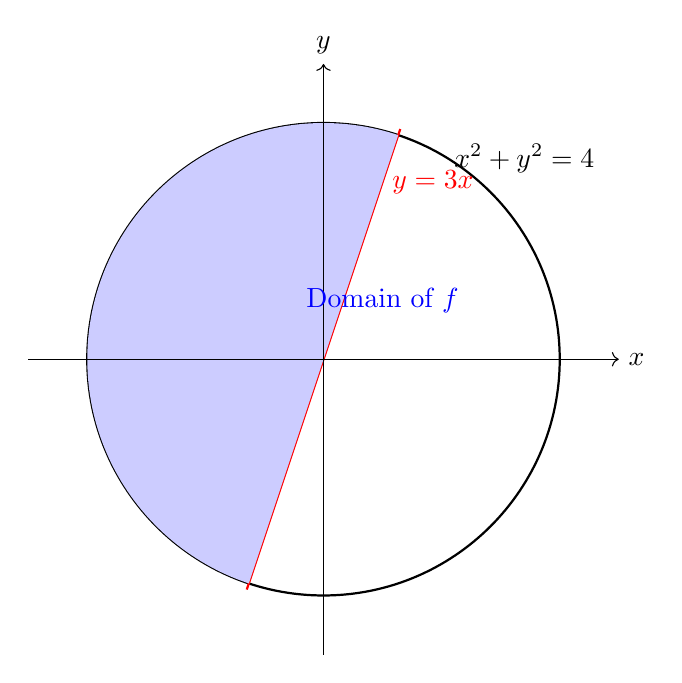
\begin{tikzpicture}[scale=1.5]
			% Draw the circle x^2 + y^2 = 4
			\draw[thick] (0,0) circle(2);
			
			% Label the circle
			\node at (1.7,1.7) {$x^2 + y^2 = 4$};
			
			% Draw the line y = 3x
			\draw[thick,red,domain=-0.65:0.65] plot (\x, {3*\x});
			
			% Label the line
			\node[red, right] at (0.5, 1.5) {$y = 3x$};
			
			% Shade the domain region
			\begin{scope}
				\clip (0,0) circle(2);
				\fill[blue!20] (-2, -6) -- (2, 6) -- (2, 2) -- (-2, 2) -- cycle;
			\end{scope}
			
			% Axes
			\draw[->] (-2.5, 0) -- (2.5, 0) node[right] {$x$};
			\draw[->] (0, -2.5) -- (0, 2.5) node[above] {$y$};
			
			% Label the domain
			\node[blue] at (0.5, 0.5) {Domain of $f$};
			
		\end{tikzpicture}
	\end{center}

	b) 
	\[ \text{Positive:} \quad  y > 3x \quad \text{and} \quad x^2 + y^{2} < 4 \] 
	\[ \text{Negative:} \quad y > 3x \quad \text{and} \quad 0 < 4 - x^{2} - y^{2} < 1 \] 
	
	
}

\newpage 
\qs{}{
	Here are several surfaces. \\
	\insertpng[0.5]{prob10a.png}
	\insertpng[0.5]{prob10b.png}
	Match each function with its graph. Justify your answers.
	\begin{enumerate}
		\item[(a)] $f(x, y) = x^2$
		\item[(b)] $f(x, y) = \sqrt{x^2 + y^2}$
		\item[(c)] $f(x, y) = e^{x^2 + y^2} - 1$
		\item[(d)] $f(x, y) = y \sin x$
		\item[(e)] $f(x, y) = \sin(x + y)$
		\item[(f)] $f(x, y) = \sin\left(\sqrt{x^2 + y^2}\right)$
	\end{enumerate}
}

\sol{
	\\
	Equation a goes with Surface V bceause it should be parabolic along the x-axis and independent of y.  \\
	Equation b goes with surface IV because the value of z should increase linearly with radical distance which should make a cone like shape \\ 
	Equation c goes with surface II z increases exponentially as x and y increase which should make for something cone like but 
	that grows faster which should make a steep smooth rise\\
	Equation d goes with surface III because the function should oscilate in the x-direction while increasing due to y values so \\
	Equation e goes with surface I because it depends on the sum of x and y and would have a constant 
	phase along lines x  + y equals a constant. So there should be a diagonal wave pattern.\\
	Equation f goes with surface VI because it should still have waves that depend on distance from origin, meaning there should be ripples. 

}
\qs{}{
	Draw a contour map of the function $f(x, y) = x^2 e^{-y}$ showing several level curves.
}

\sol{
	\[ f(x,y) = x^{2}e^{-y} \] 
	\[ x^{2}e^{-y} = k \]
	\[ e^{-y} = \frac{k}{x^{2}} \]
	\[ \ln\left( e^{-y}\right) = \ln \left( \frac{k}{x^{2}} \right)\]   
	\[ -y = \ln(k) - \ln(x^{2}) \Rightarrow y = - \ln(k) + 2\ln(x) \]
	$x^{2} > 0$ for all x in the orignal function defintion so the equation is actually 
	\[ -y = \ln(k) - \ln(x^{2}) \Rightarrow y = - \ln(k) + 2\ln(|x|) \]
	\begin{center}
		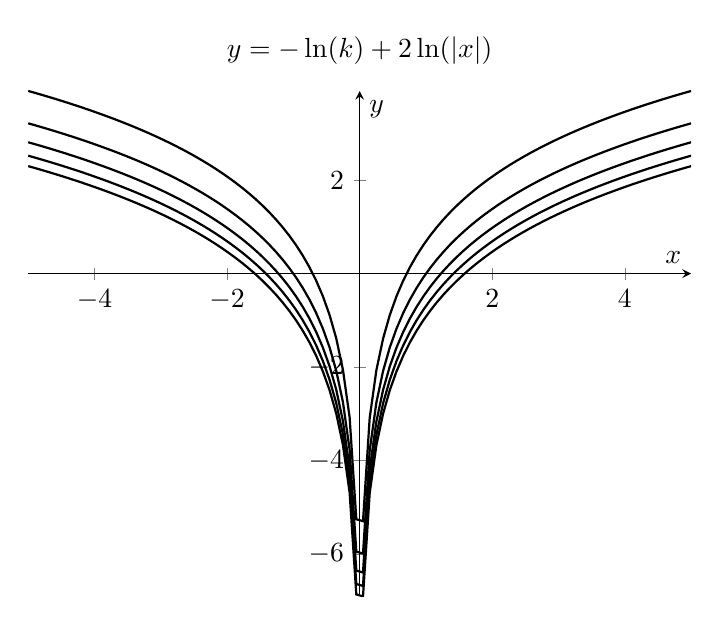
\begin{tikzpicture}
			\begin{axis}[
				axis lines = center,
				xlabel = {$x$},
				ylabel = {$y$},
				domain=-5:5,
				samples=100,
				width=10cm,
				height=8cm,
				title={$y = -\ln(k) + 2\ln(|x|)$}
			]
			% Draw several contour curves for different values of k
			\addplot [no marks, samples y=0, thick] { -ln(0.5) + 2*ln(abs(x)) }; 
			\addplot [no marks, samples y=0, thick] { -ln(1) + 2*ln(abs(x)) }; 
			\addplot [no marks, samples y=0, thick] { -ln(1.5) + 2*ln(abs(x)) }; 
			\addplot [no marks, samples y=0, thick] { -ln(2) + 2*ln(abs(x)) }; 
			\addplot [no marks, samples y=0, thick] { -ln(2.5) + 2*ln(abs(x)) }; 
			\end{axis}
		\end{tikzpicture}
	\end{center}
}

\newpage 

\qs{}{
	Match the function with its graph (labeled A-F below) and with its contour map (labeled I-VI). Give reasons for your choices.
	\begin{enumerate}
		\item[(a)] $z = e^x \cos y$
		\item[(b)] $z = \sin x - \sin y$
		\item[(c)] $z = \frac{x - y}{1 + x^2 + y^2}$
	\end{enumerate}
	\insertpng[0.6]{q12.png}
}

\newpage

\sol{\\
	a) \\
	$e^{x}$ is an exponential function in the $x$-direction, meaning that as $x$ increases the value of $z$ grow rapidly. \\
	$\cos(y)$ means that there are oscillations in the y-direction causing wave-like behavior along the $y$-axis. \\
	Graph A shows an exponential rise in the $x$-direction with some oscillations in the $y$-direction. Countour IV because of the oscillations and 
	because it is what graph A would look like from the top.  
	\\ 
	\\
	b) $\sin x - \sin y$ would have oscillations along the $x$-direction and $y$-direction. These oscillations would be of the same size as there are fixed values that 
	this equation can result in. \\
	The graph is E for this reason. Contour is III because it is a top view of the graph E and the circles are the same size which is a trait you would 
	expect.
	\\
	\\
	c)\\
	numerator of $x-y$ suggests a linear slope or difference between $x$ and $y$, so one side will be positive and the other negative. \\
	The denominator makes the effect of the numerator decrease as x and y increase since it outgrows them. So the graph of this function will have a positive peak and a negative peak near the origin 
	and then it should level out on the sides.\\
	This is why the graph is D. It is contour v because of the increasing size of the ring-like shapes as you move away from the origin which is a trait of graph d. 
}

\end{document}
